\chapter{Alberi}

\section{Introduzione}

Gli alberi sono tra le strutture dati più importanti e versatili in informatica. A differenza delle strutture lineari (array, liste, stack, code), gli alberi organizzano i dati in modo \textbf{gerarchico}, riflettendo naturalmente relazioni di tipo "padre-figlio" che occorrono in innumerevoli contesti: filesystem, organizzazioni aziendali, documenti HTML, alberi sintattici, e molto altro.

In questo capitolo studieremo alberi binari, alberi binari di ricerca (BST), alberi AVL auto-bilancianti, e heap.

\section{Alberi: definizioni fondamentali}

\subsection{Definizione matematica}

\begin{definizione}[Albero]
Un \textbf{albero} è un grafo connesso aciclico. Equivalentemente, è una collezione di nodi con le seguenti proprietà:
\begin{itemize}
    \item Esiste un nodo speciale chiamato \textbf{radice} (root)
    \item Ogni nodo diverso dalla radice ha esattamente un \textbf{padre}
    \item Non ci sono cicli
\end{itemize}
\end{definizione}

\begin{definizione}[Terminologia degli alberi]
\begin{itemize}
    \item \textbf{Radice}: Nodo senza padre
    \item \textbf{Foglia}: Nodo senza figli
    \item \textbf{Nodo interno}: Nodo con almeno un figlio
    \item \textbf{Sottoalbero}: Albero formato da un nodo e tutti i suoi discendenti
    \item \textbf{Profondità} di un nodo: Numero di archi dalla radice al nodo
    \item \textbf{Altezza} di un nodo: Numero massimo di archi dal nodo a una foglia
    \item \textbf{Altezza dell'albero}: Altezza della radice
    \item \textbf{Livello $k$}: Insieme di nodi a profondità $k$
\end{itemize}
\end{definizione}

\textbf{Visualizzazione:}

\begin{center}
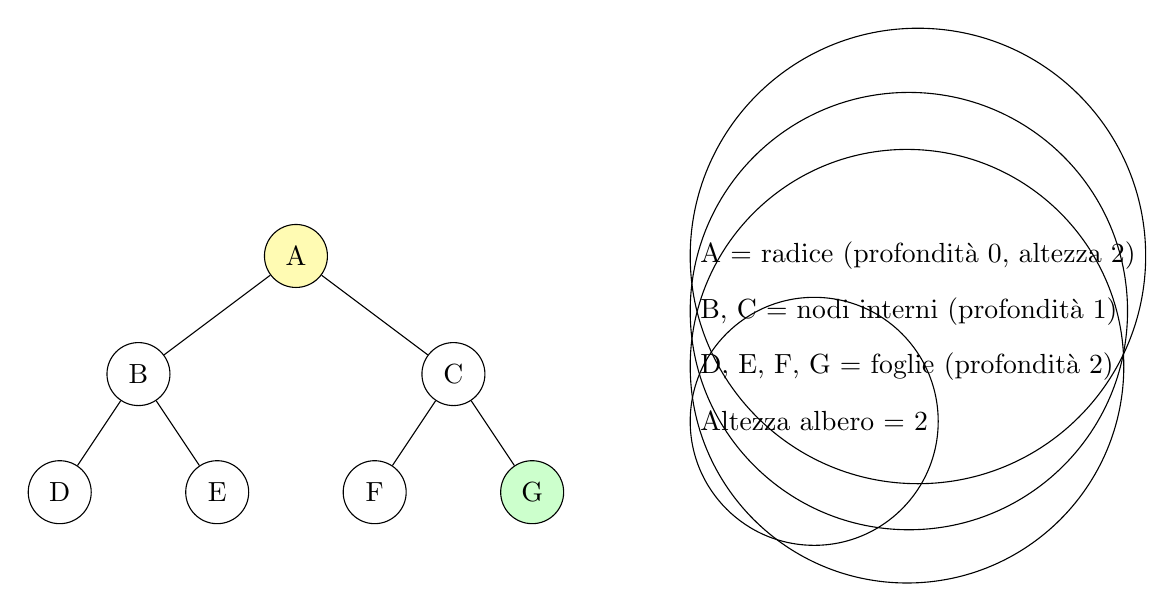
\begin{tikzpicture}[
    level distance=1.5cm,
    level 1/.style={sibling distance=4cm},
    level 2/.style={sibling distance=2cm},
    every node/.style={circle, draw, minimum size=0.8cm}
]
\node[fill=yellow!30] {A}
    child {node {B}
        child {node {D}}
        child {node {E}}
    }
    child {node {C}
        child {node {F}}
        child {node[fill=green!20] {G}}
    };

\node[right] at (5, 0) {A = radice (profondità 0, altezza 2)};
\node[right] at (5, -0.7) {B, C = nodi interni (profondità 1)};
\node[right] at (5, -1.4) {D, E, F, G = foglie (profondità 2)};
\node[right] at (5, -2.1) {Altezza albero = 2};
\end{tikzpicture}
\end{center}

\begin{teorema}[Proprietà degli alberi]
Sia $T$ un albero con $n$ nodi. Allora:
\begin{enumerate}
    \item $T$ ha esattamente $n-1$ archi
    \item Esiste un unico cammino tra qualsiasi coppia di nodi
    \item Rimuovendo un qualsiasi arco, $T$ diventa disconnesso
    \item Aggiungendo un arco tra due nodi, si crea un ciclo
\end{enumerate}
\end{teorema}

\begin{proof}[Dimostrazione del punto 1]
Per induzione su $n$.

\textbf{Caso base:} $n = 1$. Un albero con un solo nodo (la radice) ha $1 - 1 = 0$ archi. ✓

\textbf{Passo induttivo:} Assumiamo la proprietà vera per alberi con $k$ nodi. Consideriamo un albero $T$ con $k+1$ nodi. Rimuoviamo una foglia $v$ (che esiste sempre se $k+1 > 1$). L'albero rimanente $T'$ ha $k$ nodi e quindi, per ipotesi induttiva, ha $k-1$ archi. Aggiungendo la foglia $v$ con il suo arco, otteniamo $k - 1 + 1 = k = (k+1) - 1$ archi. ✓
\end{proof}

\section{Alberi binari}

\begin{definizione}[Albero binario]
Un \textbf{albero binario} è un albero in cui ogni nodo ha al massimo due figli, distinti come \textbf{figlio sinistro} e \textbf{figlio destro}.
\end{definizione}

\textbf{Struttura del nodo:}

\begin{lstlisting}[style=pseudocode]
class NodoBinario:
    def __init__(self, valore):
        self.valore = valore
        self.sinistro = None
        self.destro = None
\end{lstlisting}

\subsection{Tipi di alberi binari}

\begin{definizione}[Albero binario completo]
Un albero binario è \textbf{completo} se tutti i livelli sono completamente riempiti, eccetto eventualmente l'ultimo, che è riempito da sinistra a destra.
\end{definizione}

\begin{definizione}[Albero binario perfetto]
Un albero binario è \textbf{perfetto} se tutti i nodi interni hanno esattamente due figli e tutte le foglie sono allo stesso livello.
\end{definizione}

\begin{definizione}[Albero binario bilanciato]
Un albero binario è \textbf{bilanciato} se per ogni nodo, le altezze dei suoi sottoalberi sinistro e destro differiscono al massimo di 1.
\end{definizione}

\textbf{Visualizzazione:}

\begin{center}
\begin{tikzpicture}[
    level distance=1.2cm,
    level 1/.style={sibling distance=3cm},
    level 2/.style={sibling distance=1.5cm},
    every node/.style={circle, draw, minimum size=0.7cm}
]
% Albero perfetto
\node at (-2, 2.5) {Perfetto};
\node {1}
    child {node {2}
        child {node {4}}
        child {node {5}}
    }
    child {node {3}
        child {node {6}}
        child {node {7}}
    };

% Albero completo
\begin{scope}[xshift=7cm]
\node at (-2, 2.5) {Completo};
\node {1}
    child {node {2}
        child {node {4}}
        child {node {5}}
    }
    child {node {3}
        child {node {6}}
        child[missing]
    };
\end{scope}

% Albero sbilanciato
\begin{scope}[xshift=14cm]
\node at (-2, 2.5) {Sbilanciato};
\node {1}
    child {node {2}
        child {node {4}
            child {node {6}}
            child[missing]
        }
        child[missing]
    }
    child {node {3}}
;
\end{scope}
\end{tikzpicture}
\end{center}

\begin{teorema}[Proprietà degli alberi binari perfetti]
Un albero binario perfetto di altezza $h$ ha:
\begin{itemize}
    \item $2^{h+1} - 1$ nodi totali
    \item $2^h$ foglie
    \item $2^h - 1$ nodi interni
\end{itemize}
\end{teorema}

\begin{proof}
Il numero di nodi a livello $k$ è $2^k$ (per $k = 0, 1, \ldots, h$).

Numero totale di nodi:
\[
n = \sum_{k=0}^{h} 2^k = 2^{h+1} - 1
\]

Le foglie sono tutte al livello $h$: $2^h$ foglie.

I nodi interni sono ai livelli $0, \ldots, h-1$:
\[
\sum_{k=0}^{h-1} 2^k = 2^h - 1
\]
\end{proof}

\subsection{Visite di alberi binari}

Le visite (o attraversamenti) sono algoritmi fondamentali per processare tutti i nodi di un albero.

\subsubsection{Visita in pre-ordine (Pre-order)}

Ordine: \textbf{Radice → Sinistro → Destro}

\begin{lstlisting}[style=pseudocode]
def PreOrdine(nodo):
    """
    Visita in pre-ordine
    Complessità: O(n)
    """
    if nodo == None:
        return

    print(nodo.valore)       // Processa radice
    PreOrdine(nodo.sinistro) // Ricorsione a sinistra
    PreOrdine(nodo.destro)   // Ricorsione a destra
\end{lstlisting}

\subsubsection{Visita in-ordine (In-order)}

Ordine: \textbf{Sinistro → Radice → Destro}

\begin{lstlisting}[style=pseudocode]
def InOrdine(nodo):
    """
    Visita in-ordine
    Complessità: O(n)
    """
    if nodo == None:
        return

    InOrdine(nodo.sinistro)  // Ricorsione a sinistra
    print(nodo.valore)       // Processa radice
    InOrdine(nodo.destro)    // Ricorsione a destra
\end{lstlisting}

\subsubsection{Visita post-ordine (Post-order)}

Ordine: \textbf{Sinistro → Destro → Radice}

\begin{lstlisting}[style=pseudocode]
def PostOrdine(nodo):
    """
    Visita post-ordine
    Complessità: O(n)
    """
    if nodo == None:
        return

    PostOrdine(nodo.sinistro) // Ricorsione a sinistra
    PostOrdine(nodo.destro)   // Ricorsione a destra
    print(nodo.valore)        // Processa radice
\end{lstlisting}

\subsubsection{Visita per livelli (Level-order / BFS)}

Usa una coda per visitare livello per livello.

\begin{lstlisting}[style=pseudocode]
def VisitaLivelli(radice):
    """
    Visita per livelli (BFS)
    Complessità: O(n)
    """
    if radice == None:
        return

    coda = Queue()
    coda.enqueue(radice)

    while not coda.isEmpty():
        nodo = coda.dequeue()
        print(nodo.valore)

        if nodo.sinistro != None:
            coda.enqueue(nodo.sinistro)

        if nodo.destro != None:
            coda.enqueue(nodo.destro)
\end{lstlisting}

\textbf{Esempio di visite:}

\begin{center}
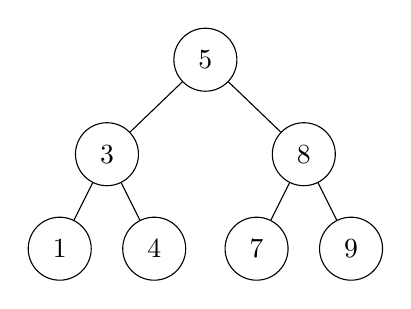
\begin{tikzpicture}[
    level distance=1.2cm,
    level 1/.style={sibling distance=2.5cm},
    level 2/.style={sibling distance=1.2cm},
    every node/.style={circle, draw, minimum size=0.8cm}
]
\node {5}
    child {node {3}
        child {node {1}}
        child {node {4}}
    }
    child {node {8}
        child {node {7}}
        child {node {9}}
    };
\end{tikzpicture}

\small
\begin{itemize}
    \item Pre-ordine: 5, 3, 1, 4, 8, 7, 9
    \item In-ordine: 1, 3, 4, 5, 7, 8, 9
    \item Post-ordine: 1, 4, 3, 7, 9, 8, 5
    \item Per livelli: 5, 3, 8, 1, 4, 7, 9
\end{itemize}
\end{center}

\section{Alberi binari di ricerca (BST)}

\begin{definizione}[Albero binario di ricerca]
Un \textbf{albero binario di ricerca} (BST) è un albero binario in cui, per ogni nodo $x$:
\begin{itemize}
    \item Tutti i nodi nel sottoalbero sinistro di $x$ hanno valori $\leq x.\text{valore}$
    \item Tutti i nodi nel sottoalbero destro di $x$ hanno valori $> x.\text{valore}$
\end{itemize}
\end{definizione}

\textbf{Proprietà fondamentale:} La visita in-ordine di un BST produce i valori in ordine crescente.

\begin{center}
\begin{tikzpicture}[
    level distance=1.5cm,
    level 1/.style={sibling distance=3.5cm},
    level 2/.style={sibling distance=1.8cm},
    every node/.style={circle, draw, minimum size=0.9cm}
]
\node {15}
    child {node {6}
        child {node {3}
            child {node {2}}
            child {node {4}}
        }
        child {node {7}
            child[missing]
            child {node {13}
                child {node {9}}
                child[missing]
            }
        }
    }
    child {node {18}
        child {node {17}}
        child {node {20}}
    };

\node[right] at (6, 0) {BST: In-ordine = 2, 3, 4, 6, 7, 9, 13, 15, 17, 18, 20};
\end{tikzpicture}
\end{center}

\subsection{Operazioni su BST}

\subsubsection{Ricerca}

\begin{lstlisting}[style=pseudocode]
def Ricerca(nodo, chiave):
    """
    Cerca una chiave nel BST
    Input: radice, chiave da cercare
    Output: nodo se trovato, None altrimenti
    Complessità: O(h) dove h = altezza
    """
    if nodo == None or nodo.valore == chiave:
        return nodo

    if chiave < nodo.valore:
        return Ricerca(nodo.sinistro, chiave)
    else:
        return Ricerca(nodo.destro, chiave)
\end{lstlisting}

\textbf{Complessità:} L'analisi della complessità della ricerca in un BST dipende fortemente dalla struttura dell'albero. Nel caso migliore, quando la chiave cercata si trova alla radice, l'operazione richiede tempo costante $O(1)$. Più in generale, la complessità nel caso peggiore è $O(h)$, dove $h$ rappresenta l'altezza dell'albero, poiché nel peggiore dei casi potremmo dover attraversare un cammino dalla radice fino a una foglia. Se l'albero è bilanciato, l'altezza è logaritmica rispetto al numero di nodi, ottenendo quindi una complessità $O(\log n)$. Tuttavia, quando l'albero è completamente sbilanciato e degenera in una struttura simile a una lista, la complessità peggiora fino a $O(n)$.

\subsubsection{Minimo e massimo}

\begin{lstlisting}[style=pseudocode]
def Minimo(nodo):
    """
    Trova il valore minimo (nodo più a sinistra)
    Complessità: O(h)
    """
    while nodo.sinistro != None:
        nodo = nodo.sinistro
    return nodo

def Massimo(nodo):
    """
    Trova il valore massimo (nodo più a destra)
    Complessità: O(h)
    """
    while nodo.destro != None:
        nodo = nodo.destro
    return nodo
\end{lstlisting}

\subsubsection{Inserimento}

\begin{lstlisting}[style=pseudocode]
def Inserisci(nodo, chiave):
    """
    Inserisce una chiave nel BST
    Complessità: O(h)
    """
    if nodo == None:
        return NodoBinario(chiave)

    if chiave < nodo.valore:
        nodo.sinistro = Inserisci(nodo.sinistro, chiave)
    elif chiave > nodo.valore:
        nodo.destro = Inserisci(nodo.destro, chiave)
    // Se chiave == nodo.valore, ignoriamo (no duplicati)

    return nodo
\end{lstlisting}

\textbf{Esempio di inserimento:}

\begin{center}
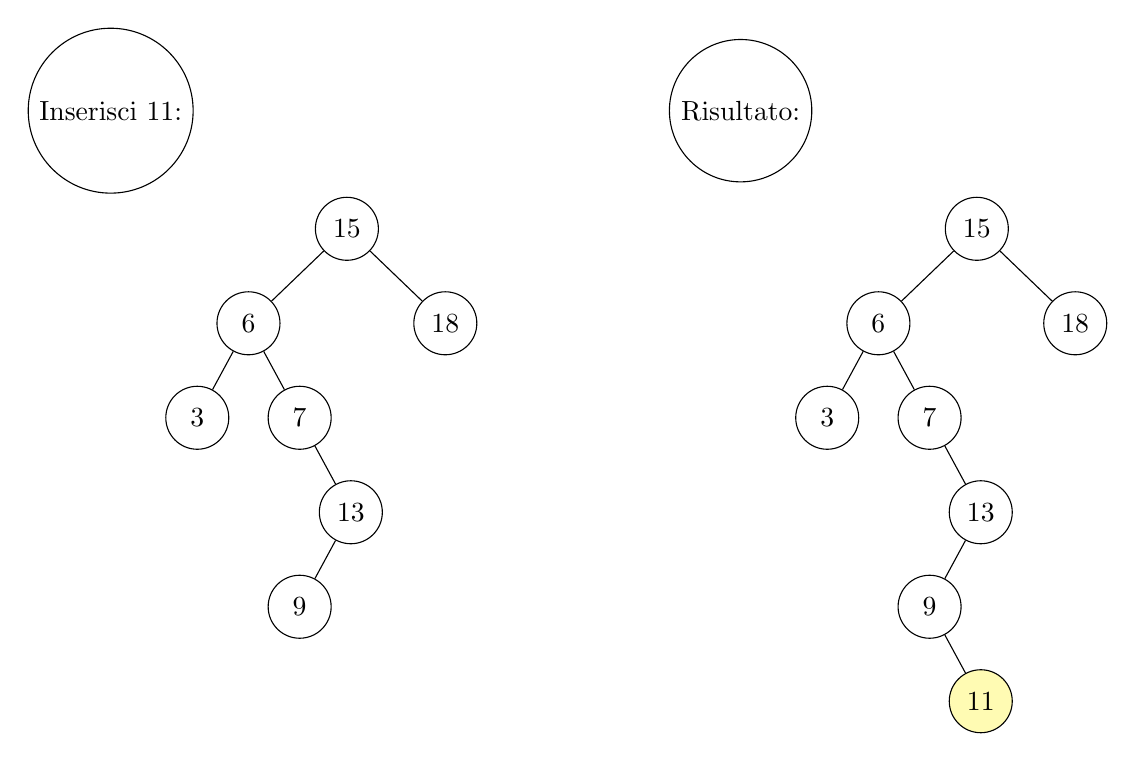
\begin{tikzpicture}[
    level distance=1.2cm,
    level 1/.style={sibling distance=2.5cm},
    level 2/.style={sibling distance=1.3cm},
    every node/.style={circle, draw, minimum size=0.8cm}
]
% Prima
\node at (-3, 1.5) {Inserisci 11:};
\node {15}
    child {node {6}
        child {node {3}}
        child {node {7}
            child[missing]
            child {node {13}
                child {node {9}}
                child[missing]
            }
        }
    }
    child {node {18}};

% Dopo
\begin{scope}[xshift=8cm]
\node at (-3, 1.5) {Risultato:};
\node {15}
    child {node {6}
        child {node {3}}
        child {node {7}
            child[missing]
            child {node {13}
                child {node {9}
                    child[missing]
                    child {node[fill=yellow!30] {11}}
                }
                child[missing]
            }
        }
    }
    child {node {18}};
\end{scope}
\end{tikzpicture}
\end{center}

\subsubsection{Cancellazione}

La cancellazione è l'operazione più complessa. Tre casi:

\begin{enumerate}
    \item \textbf{Nodo foglia}: Rimuoviamo semplicemente il nodo
    \item \textbf{Nodo con un figlio}: Sostituiamo il nodo con il suo unico figlio
    \item \textbf{Nodo con due figli}: Sostituiamo il nodo con il suo \textit{successore} (il minimo del sottoalbero destro) o \textit{predecessore} (il massimo del sottoalbero sinistro)
\end{enumerate}

\begin{lstlisting}[style=pseudocode]
def Cancella(nodo, chiave):
    """
    Cancella una chiave dal BST
    Complessità: O(h)
    """
    if nodo == None:
        return None

    if chiave < nodo.valore:
        nodo.sinistro = Cancella(nodo.sinistro, chiave)
    elif chiave > nodo.valore:
        nodo.destro = Cancella(nodo.destro, chiave)
    else:
        // Nodo trovato, cancelliamolo
        // Caso 1: Foglia o un solo figlio
        if nodo.sinistro == None:
            return nodo.destro
        elif nodo.destro == None:
            return nodo.sinistro

        // Caso 2: Due figli
        // Trova il successore (minimo del sottoalbero destro)
        successore = Minimo(nodo.destro)
        nodo.valore = successore.valore
        nodo.destro = Cancella(nodo.destro, successore.valore)

    return nodo
\end{lstlisting}

\subsection{Analisi delle prestazioni dei BST}

\begin{center}
\begin{tabular}{|l|c|c|}
\hline
\textbf{Operazione} & \textbf{Caso medio} & \textbf{Caso peggiore} \\
\hline
Ricerca & $O(\log n)$ & $O(n)$ \\
Inserimento & $O(\log n)$ & $O(n)$ \\
Cancellazione & $O(\log n)$ & $O(n)$ \\
Minimo/Massimo & $O(\log n)$ & $O(n)$ \\
\hline
\end{tabular}
\end{center}

Il caso peggiore si verifica quando l'albero è completamente sbilanciato (degenera in lista).

\section{Alberi AVL (Auto-bilancianti)}

Il problema dei BST sbilanciati è risolto dagli \textbf{alberi AVL}, che mantengono l'albero bilanciato automaticamente.

\begin{definizione}[Albero AVL]
Un albero AVL è un BST in cui, per ogni nodo, le altezze dei sottoalberi sinistro e destro differiscono al massimo di 1.
\end{definizione}

\textbf{Fattore di bilanciamento:}
\[
BF(nodo) = \text{altezza(sinistro)} - \text{altezza(destro)} \in \{-1, 0, 1\}
\]

\subsection{Rotazioni}

Per mantenere il bilanciamento, gli alberi AVL usano le \textbf{rotazioni}.

\subsubsection{Rotazione sinistra (Left Rotation)}

\begin{center}
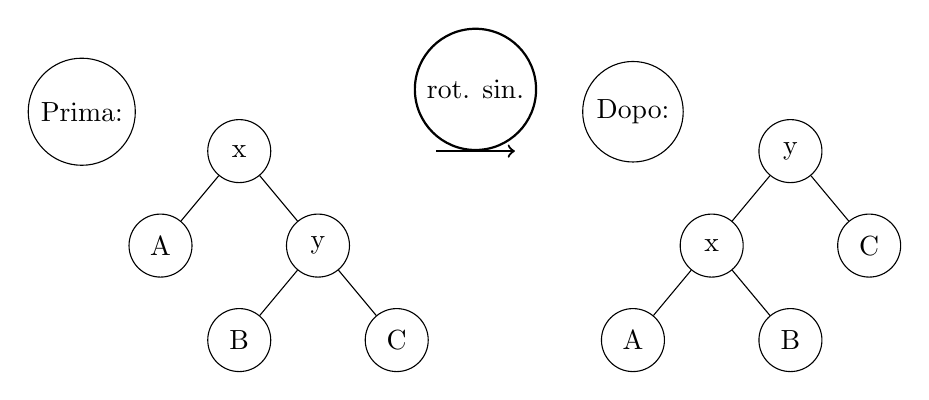
\begin{tikzpicture}[
    every node/.style={circle, draw, minimum size=0.8cm},
    level distance=1.2cm,
    level 1/.style={sibling distance=2cm}
]
% Prima
\node at (-2, 0.5) {Prima:};
\node (x) {x}
    child {node {A}}
    child {node (y) {y}
        child {node {B}}
        child {node {C}}
    };

\draw[->, thick] (2.5, 0) -- (3.5, 0) node[midway, above] {rot. sin.};

% Dopo
\begin{scope}[xshift=7cm]
\node at (-2, 0.5) {Dopo:};
\node (y2) {y}
    child {node (x2) {x}
        child {node {A}}
        child {node {B}}
    }
    child {node {C}};
\end{scope}
\end{tikzpicture}
\end{center}

\begin{lstlisting}[style=pseudocode]
def RotazioneSinistra(x):
    """
    Rotazione sinistra attorno a x
    Complessità: O(1)
    """
    y = x.destro
    B = y.sinistro

    // Effettua rotazione
    y.sinistro = x
    x.destro = B

    // Aggiorna altezze
    x.altezza = 1 + max(altezza(x.sinistro), altezza(x.destro))
    y.altezza = 1 + max(altezza(y.sinistro), altezza(y.destro))

    return y  // nuova radice
\end{lstlisting}

\subsubsection{Rotazione destra (Right Rotation)}

Simmetrica alla rotazione sinistra.

\begin{lstlisting}[style=pseudocode]
def RotazioneDestra(y):
    """
    Rotazione destra attorno a y
    Complessità: O(1)
    """
    x = y.sinistro
    B = x.destro

    // Effettua rotazione
    x.destro = y
    y.sinistro = B

    // Aggiorna altezze
    y.altezza = 1 + max(altezza(y.sinistro), altezza(y.destro))
    x.altezza = 1 + max(altezza(x.sinistro), altezza(x.destro))

    return x  // nuova radice
\end{lstlisting}

\subsection{Quattro casi di sbilanciamento}

\begin{enumerate}
    \item \textbf{Left-Left (LL)}: Risolto con rotazione destra
    \item \textbf{Right-Right (RR)}: Risolto con rotazione sinistra
    \item \textbf{Left-Right (LR)}: Risolto con rotazione sinistra sul figlio sinistro, poi rotazione destra
    \item \textbf{Right-Left (RL)}: Risolto con rotazione destra sul figlio destro, poi rotazione sinistra
\end{enumerate}

\subsection{Inserimento in AVL}

\begin{lstlisting}[style=pseudocode]
def InserisciAVL(nodo, chiave):
    """
    Inserimento in albero AVL con bilanciamento
    Complessità: O(log n)
    """
    // 1. Inserimento BST normale
    if nodo == None:
        return NodoBinario(chiave)

    if chiave < nodo.valore:
        nodo.sinistro = InserisciAVL(nodo.sinistro, chiave)
    else:
        nodo.destro = InserisciAVL(nodo.destro, chiave)

    // 2. Aggiorna altezza
    nodo.altezza = 1 + max(altezza(nodo.sinistro), altezza(nodo.destro))

    // 3. Calcola fattore di bilanciamento
    bf = altezza(nodo.sinistro) - altezza(nodo.destro)

    // 4. Bilancia se necessario
    // Caso Left-Left
    if bf > 1 and chiave < nodo.sinistro.valore:
        return RotazioneDestra(nodo)

    // Caso Right-Right
    if bf < -1 and chiave > nodo.destro.valore:
        return RotazioneSinistra(nodo)

    // Caso Left-Right
    if bf > 1 and chiave > nodo.sinistro.valore:
        nodo.sinistro = RotazioneSinistra(nodo.sinistro)
        return RotazioneDestra(nodo)

    // Caso Right-Left
    if bf < -1 and chiave < nodo.destro.valore:
        nodo.destro = RotazioneDestra(nodo.destro)
        return RotazioneSinistra(nodo)

    return nodo
\end{lstlisting}

\begin{teorema}[Complessità AVL]
In un albero AVL con $n$ nodi:
\begin{itemize}
    \item L'altezza è $O(\log n)$
    \item Ricerca, inserimento, cancellazione richiedono $O(\log n)$ nel caso peggiore
\end{itemize}
\end{teorema}

\section{Heap}

\begin{definizione}[Heap]
Un \textbf{heap} è un albero binario quasi completo che soddisfa la \textbf{proprietà di heap}:
\begin{itemize}
    \item \textbf{Max-heap}: Ogni nodo ha valore $\geq$ dei suoi figli
    \item \textbf{Min-heap}: Ogni nodo ha valore $\leq$ dei suoi figli
\end{itemize}
\end{definizione}

\textbf{Visualizzazione di un max-heap:}

\begin{center}
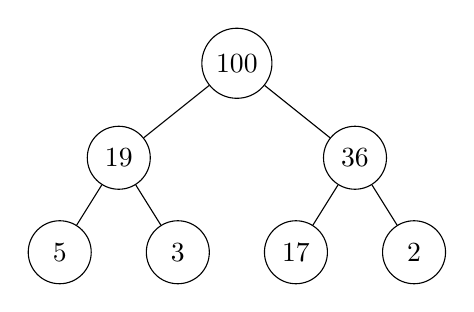
\begin{tikzpicture}[
    level distance=1.2cm,
    level 1/.style={sibling distance=3cm},
    level 2/.style={sibling distance=1.5cm},
    every node/.style={circle, draw, minimum size=0.8cm}
]
\node {100}
    child {node {19}
        child {node {5}}
        child {node {3}}
    }
    child {node {36}
        child {node {17}}
        child {node {2}}
    };
\end{tikzpicture}
\end{center}

\subsection{Rappresentazione con array}

Gli heap sono implementati efficientemente con array, sfruttando la proprietà di essere quasi completi.

Per un nodo in posizione $i$ (partendo da 1):
\begin{itemize}
    \item Padre: $\lfloor i/2 \rfloor$
    \item Figlio sinistro: $2i$
    \item Figlio destro: $2i + 1$
\end{itemize}

\begin{center}
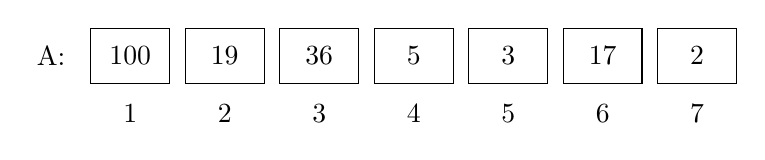
\begin{tikzpicture}
    % Array
    \foreach \i/\val in {1/100, 2/19, 3/36, 4/5, 5/3, 6/17, 7/2} {
        \node[rectangle, draw, minimum width=1cm, minimum height=0.7cm] at (\i*1.2, 0) {\val};
        \node[below] at (\i*1.2, -0.5) {\i};
    }

    \node[left] at (0.5, 0) {A:};
\end{tikzpicture}
\end{center}

\subsection{Operazioni su heap}

\subsubsection{Heapify (Ripristina proprietà heap)}

\begin{lstlisting}[style=pseudocode]
def MaxHeapify(A, i, heap_size):
    """
    Ripristina la proprietà di max-heap
    Assumendo che i sottoalberi siano già heap validi
    Complessità: O(log n)
    """
    sinistro = 2 * i
    destro = 2 * i + 1
    massimo = i

    if sinistro <= heap_size and A[sinistro] > A[massimo]:
        massimo = sinistro

    if destro <= heap_size and A[destro] > A[massimo]:
        massimo = destro

    if massimo != i:
        scambia A[i] con A[massimo]
        MaxHeapify(A, massimo, heap_size)
\end{lstlisting}

\subsubsection{Costruzione heap}

\begin{lstlisting}[style=pseudocode]
def CostruisciMaxHeap(A, n):
    """
    Costruisce un max-heap da un array non ordinato
    Complessità: O(n)  // Non O(n log n)!
    """
    heap_size = n
    // Partiamo dall'ultimo nodo non-foglia e andiamo indietro
    for i = n/2 down to 1:
        MaxHeapify(A, i, heap_size)
\end{lstlisting}

\begin{teorema}[Complessità di CostruisciMaxHeap]
La costruzione di un heap da un array di $n$ elementi richiede $O(n)$ tempo.
\end{teorema}

\begin{proof}[Idea]
Il numero di nodi a livello $h$ è al massimo $\lceil n/2^{h+1} \rceil$, e l'altezza di questi nodi è $h$.

Il costo totale è:
\[
\sum_{h=0}^{\lfloor \log n \rfloor} \lceil n/2^{h+1} \rceil \cdot O(h) = O\left(n \sum_{h=0}^{\infty} \frac{h}{2^h}\right) = O(n)
\]

dove abbiamo usato $\sum_{h=0}^{\infty} \frac{h}{2^h} = 2$.
\end{proof}

\subsubsection{Inserimento}

\begin{lstlisting}[style=pseudocode]
def InserisciHeap(A, heap_size, chiave):
    """
    Inserisce una chiave nel max-heap
    Complessità: O(log n)
    """
    heap_size = heap_size + 1
    i = heap_size
    A[i] = -∞

    // Risali verso la radice finché la proprietà heap è violata
    while i > 1 and A[i/2] < chiave:
        A[i] = A[i/2]
        i = i / 2

    A[i] = chiave
    return heap_size
\end{lstlisting}

\subsubsection{Estrazione del massimo}

\begin{lstlisting}[style=pseudocode]
def EstraiMassimo(A, heap_size):
    """
    Estrae e restituisce il massimo (radice)
    Complessità: O(log n)
    """
    if heap_size < 1:
        errore "Heap underflow"

    max = A[1]
    A[1] = A[heap_size]
    heap_size = heap_size - 1
    MaxHeapify(A, 1, heap_size)

    return max, heap_size
\end{lstlisting}

\subsection{Applicazione: Heap Sort}

\begin{lstlisting}[style=pseudocode]
def HeapSort(A, n):
    """
    Ordinamento con heap
    Complessità: O(n log n) tempo, O(1) spazio
    """
    CostruisciMaxHeap(A, n)
    heap_size = n

    for i = n down to 2:
        scambia A[1] con A[i]
        heap_size = heap_size - 1
        MaxHeapify(A, 1, heap_size)
\end{lstlisting}

\textbf{Complessità:} $O(n \log n)$ nel caso peggiore, $O(1)$ spazio ausiliario.

\section{Tabella riassuntiva}

\begin{center}
\begin{tabular}{|l|c|c|c|}
\hline
\textbf{Operazione} & \textbf{BST} & \textbf{AVL} & \textbf{Heap} \\
\hline
Ricerca & $O(n)$ worst & $O(\log n)$ & $O(n)$ \\
Inserimento & $O(n)$ worst & $O(\log n)$ & $O(\log n)$ \\
Cancellazione & $O(n)$ worst & $O(\log n)$ & $O(\log n)$ \\
Trova min/max & $O(n)$ worst & $O(\log n)$ & $O(1)$ \\
Costruzione & $O(n \log n)$ & $O(n \log n)$ & $O(n)$ \\
In-order traversal & Ordinato & Ordinato & Non ordinato \\
\hline
\end{tabular}
\end{center}

\section{Conclusioni}

Gli alberi sono strutture dati potentissime con applicazioni vastissime. I \textbf{BST} (alberi binari di ricerca) trovano impiego naturale nell'implementazione di dizionari, insiemi ordinati e database indicizzati, dove è fondamentale mantenere i dati ordinati consentendo ricerche efficienti. Gli \textbf{alberi AVL} sono la scelta preferita quando è necessario garantire prestazioni ottimali anche nel caso peggiore, grazie al loro bilanciamento automatico che mantiene l'altezza logaritmica. Gli \textbf{heap}, invece, sono ideali per implementare code con priorità e trovano applicazione cruciale nell'algoritmo di ordinamento HeapSort e in algoritmi su grafi come Dijkstra e Prim, dove è essenziale estrarre efficientemente l'elemento con priorità massima o minima.

\textbf{Punti chiave:} I concetti fondamentali da ricordare sugli alberi riguardano innanzitutto la proprietà caratteristica dei BST, per cui la visita in-ordine produce sempre una sequenza ordinata degli elementi. Gli alberi AVL si distinguono per il loro meccanismo di bilanciamento automatico, realizzato attraverso operazioni di rotazione che mantengono la struttura bilanciata dopo ogni inserimento o cancellazione. Gli heap, invece, si caratterizzano per la proprietà di heap (max o min) e per la loro efficiente rappresentazione mediante array, che consente di navigare facilmente tra nodi padre e figli. Un aspetto cruciale comune a tutte queste strutture è che la complessità delle operazioni dipende strettamente dall'altezza dell'albero: è proprio per questo motivo che gli alberi bilanciati sono così importanti, poiché garantiscono un'altezza logaritmica e quindi una complessità $O(\log n)$ per le operazioni principali.
